% !TeX program = lualatex
% !TeX encoding = utf8
% !TeX spellcheck = uk_UA
% !TeX root =../MexPractEng.tex

%=========================================================
\chapter{Rigid body dynamics}\label{\currfilebase}
\Opensolutionfile{answer}[\currfilebase/\currfilebase-Answers]
\Writetofile{answer}{\protect\section*{\nameref*{\currfilebase}}}%
%=========================================================

\section{Calculating the Rotational Inertia}

%=========================================================
\begin{problem}\label{prb:rot_inertia_of_disk}
	Figure~\ref{rot_inertia_of_disk_a} shows a disk that can rotate about an axis at a radial distance $h$ from the center of the disk. Figure~\ref{rot_inertia_of_disk_b} gives the rotational inertia (momentum of inertia) $I$ of the disk about the axis as a function of that distance $h$, from the center out to the edge of the disk. 
	\begin{enumerate*}[label=(\alph*)]
		\item 	What is the mass of the disk?
		\item 	What is the radius of the disk?
	\end{enumerate*}
	\begin{solution}
		\begin{enumerate*}[label=(\alph*)]
			\item $2.5$~\si{\kilo\gram};
			\item $\approx 0.63$~\si{\meter}.
		\end{enumerate*}
	\end{solution}
\end{problem}

%=========================================================
\begin{figure}[h!]\centering
	%---------------------------------------------------------
	\begin{subfigure}[t]{0.45\linewidth}\centering
		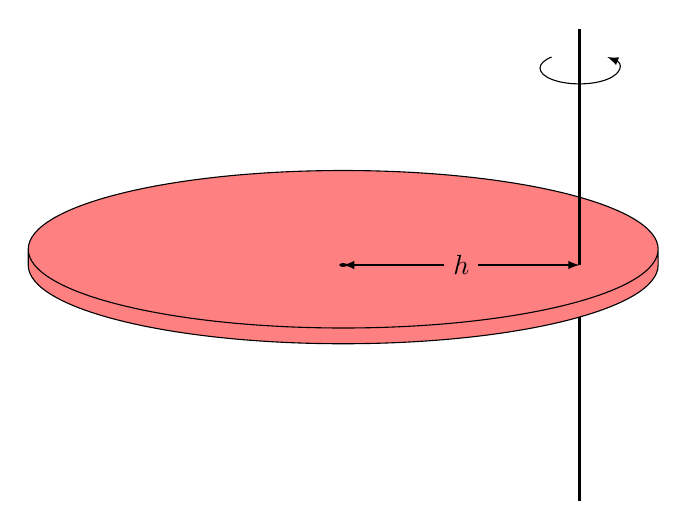
\begin{tikzpicture}
			\pgfmathsetmacro{\dl}{3}
			\pgfmathsetmacro{\a}{4}
			\pgfmathsetmacro{\b}{1}
			\pgfmathsetmacro{\h}{6}
			\pgfmathsetmacro{\th}{0.2}
			\draw[thick] (\dl,-{\h/2}) -- (\dl,0);
			\fill[red!50, draw=black] (-\a,\th) -- (-\a,0) arc (180:360:\a{} and \b) -- +(0,\th) arc (0:-180:\a{} and \b) arc (180:0:\a{} and \b) arc (0:-180:\a{} and \b);
			\draw[thick] (\dl,0) -- (\dl,{\h/2});
			\fill (0,0) ellipse (0.05 and 0.025);
			\draw[latex-latex] (0,0) -- node[fill = red!50] {$h$} (\dl,0);
			\draw[-latex] (\dl,{\h/2-0.5}) +(-225:0.5 and 0.2) arc (-225:45:0.5 and 0.2);
		\end{tikzpicture}
		\caption{}
		\label{rot_inertia_of_disk_a}
	\end{subfigure}
	%---------------------------------------------------------
	\begin{subfigure}[t]{0.45\linewidth}\centering
		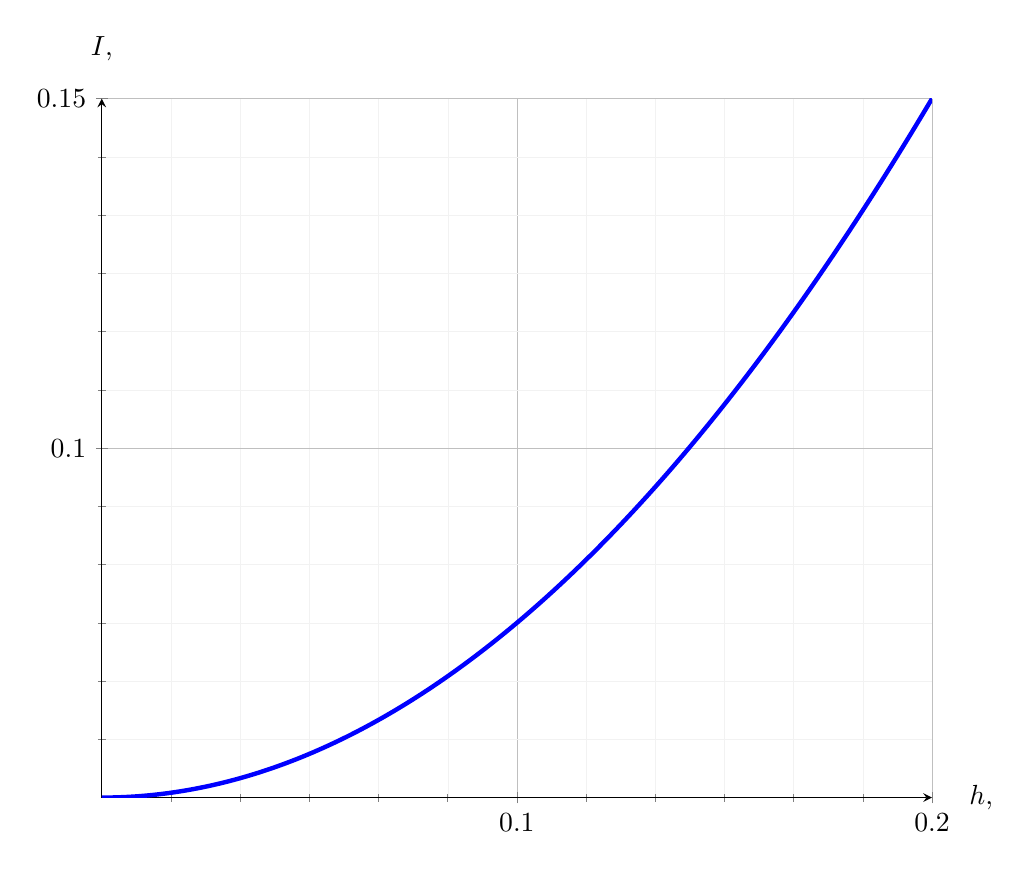
\begin{tikzpicture}
			\begin{axis}[%
			% === Налаштування сітки ===
			grid = both,
			grid style={line width=.1pt, draw=gray!10},
			major grid style={line width=.2pt,draw=gray!50},
			minor tick num = 5,
			minor grid style = {line width=.1pt,draw=gray!10},
			% === Налаштування положення координатних осей ===
			axis lines = middle,
			axis line style={-stealth},
			% === Вибір підписів шкали для відображення ===
			xtick = {0,0.1,0.2},
			ytick = {0.05,0.1,0.15},
			% === Підпис координатних осей ===
			xlabel={$h$, \si{\meter}},
			ylabel={$I$, \si{\kilo\gram\square\meter}},
			% === Положення підпису координатних осей ===
			xlabel style={right = 10pt},
			ylabel style={above = 10pt},
			% === Налаштування мінімальних та максимальних значень координат ===
			xmin = 0,
			xmax =  0.2,
			ymin = 0.050,
			ymax =  0.150,
			% === Налаштування розміру графіка ===
			width=\linewidth,
			]
			\addplot+[blue, no marks, domain={0:0.2}, samples=500, ultra thick] {2.5*x^2+0.05};
			\end{axis}
		\end{tikzpicture}
		\caption{}
		\label{rot_inertia_of_disk_b}
	\end{subfigure}
	%---------------------------------------------------------
	\caption{Problem~\ref{prb:rot_inertia_of_disk}}
	\label{rot_inertia_of_disk}
\end{figure}
%=========================================================


%=========================================================
\begin{problem}\label{prb:rot_combination}
	In Fig.~\ref{rot_combination}, two particles, each with mass $m = 0.85$~kg, are fastened to each other, and to a rotation axis at $O$, by two thin rods, each with length $d = 5.6$~cm and mass $M = 1.2$~kg. The combination rotates around the rotation axis with the angular speed $v = 0.30$~rad/s. Measured about $O$, what are the combination’s 
	\begin{enumerate*}[label=(\alph*)]
		\item rotational inertia and
		\item kinetic energy?
	\end{enumerate*}
	\begin{solution}
		\begin{enumerate*}[label=(\alph*)]
			\item $0.023$~\si{\kilo\gram\square\meter},
			\item $1.1$~\si{\milli\joule}.
		\end{enumerate*}
	\end{solution}
\end{problem}

%---------------------------------------------------------
\begin{figure}[h!]\centering
	\begin{tikzpicture}
		% ------ parameters -------------
		\pgfmathsetmacro{\l}{8}
		\pgfmathsetmacro{\R}{0.4}
		\coordinate (B1) at (\l/2,0);
		\coordinate (B2) at (\l,0);
		\coordinate (O) at (0,0);
		\fill (O) circle (0.1);
		\draw[ultra thick] (O) -- (\l,0);
		\draw[ball color = red!50] (B1) circle (\R);
		\draw[ball color = red!50] (B2) circle (\R);
		% -------- nodes -------
		\node at (B1) {$m$};
		\node at (B2) {$m$};
		\node[above] at ($(O)!0.5!(B1)$) {$d$};\node[below] at ($(O)!0.5!(B1)$) {$M$};
		\node[above] at ($(B1)!0.5!(B2)$) {$d$};\node[below] at ($(B1)!0.5!(B2)$) {$M$};
		\draw[-latex, thick, cyan] (O) +(-225:0.5) arc (-225:45:0.5) node[above, text=black] {$\omega$};
	\end{tikzpicture}
	\caption{Problem~\ref{prb:rot_combination}}
	\label{rot_combination}
\end{figure}
%---------------------------------------------------------

\section{Newton's Second Law for Rotation}

%=========================================================
\begin{problem}\label{prb:rot_single_disk}
	Figure~\ref{rot_single_disk} shows a uniform disk that can rotate around its center. The disk has a radius of $2.00$~cm and a mass of $20.0$~g and is initially at rest. Starting at time $t = 0$, two forces are to be applied tangentially to the rim as indicated, so that at time $t = 1.25$~s the disk has an angular velocity of $250$~rad/s counterclockwise. Force $\vec F_1$ has a magnitude of $0.100$~N. What is magnitude $F_2$?
	\begin{solution}
		$0.140$~\si{\newton}.
	\end{solution}
\end{problem}


%=========================================================
\begin{problem}\label{prb:rot_Athwood}
	In Fig.~\ref{rot_Athwood}, block 1 has mass $m_1 = 460$~g, block 2 has mass $m_2 = 500$~g, and the pulley, which is mounted on a horizontal axle with negligible friction, has radius $R = 5.00$~cm. When released from rest, block 2 falls $75.0$~cm in $5.00$~s without the cord slipping on the pulley. 
	\begin{enumerate*}[label=(\alph*)]
		\item What is the magnitude of the acceleration of the blocks?
		What are 
		\item tension $T_2$
		and 
		\item tension $T_1$?
		\item What is the magnitude of the pulley’s angular acceleration?
		\item What is its rotational inertia?
	\end{enumerate*}
	\begin{solution}
		\begin{enumerate*}[label=(\alph*)]
			\item $6.00$~\si{\centi\meter\per\square\second};
			\item $4.87$~\si{\newton}; 
			\item $4.54$~\si{\newton}; 
			\item $1.20$~\si{\radian\per\square\second}; 
			\item $0.0138$~\si{\kilo\gram\square\meter}.
		\end{enumerate*}
	\end{solution}
\end{problem}

	%=========================================================
	\begin{figure}[h!]\centering
		%---------------------------------------------------------
		\begin{minipage}[t]{0.45\linewidth}\centering
			\begin{tikzpicture}
				\pgfmathsetmacro{\R}{1.5}
				\draw[fill=orange!50, thick] (0,0) circle (\R);
				\fill[] (0,0) circle (0.05);
				\coordinate (O) at (0,0);
				\pgfmathsetmacro{\bangle}{45}
				\coordinate (F1) at ({180-\bangle}:\R);
				\coordinate (F2) at (45:\R);
				\draw[dashed] (O) -- (F1);
				\draw[dashed] (O) -- (F2);
				\draw[-latex, thick, cyan] (F1) -- ($(F1)!1.5cm!-90:(O)$) coordinate (F1E) node[text=black, left] {$\vec F_1$};
				\draw[-latex, thick, cyan] (F2) -- ($(F2)!2cm!90:(O)$)  coordinate (F2E) node[text=black, right] {$\vec F_2$};
				\draw [right angle length=0.2cm, right angle quadrant=1, right angle symbol={F1E}{F1}{O}];
				\draw [right angle length=0.2cm, right angle quadrant=1, right angle symbol={F2E}{F2}{O}];
			\end{tikzpicture}
			\caption{Problem~\ref{prb:rot_single_disk}}
			\label{rot_single_disk}
		\end{minipage}
		%---------------------------------------------------------
		\begin{minipage}[t]{0.45\linewidth}\centering
			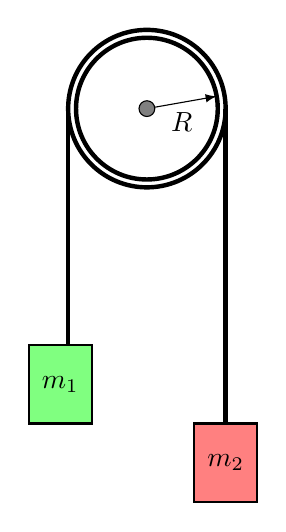
\begin{tikzpicture}
			\draw[ultra thick, fill=white] (0.0,10) circle (1);
			\draw[ultra thick] (0.0,10) circle (0.9);
			\draw[-latex] (0,10) -- node[below] {$R$} +(10:0.9);
			\draw[fill=gray] (0.0,10) circle (0.1);
			\draw[ultra thick] (-1,10) -- (-1,7);
			\draw[thick, fill=green!50] (-1.5,7) rectangle node {$m_1$} +(0.8,-1);
			\coordinate (B) at (1,6);
			\draw[ultra thick] (1,10) --  (B);
			\draw[thick, fill=red!50] ([shift={(-0.4,0)}]B) rectangle node {$m_2$} +(0.8,-1);
			\end{tikzpicture}
			\caption{Problem~\ref{prb:rot_Athwood}}
			\label{rot_Athwood}
		\end{minipage}
		%---------------------------------------------------------
	\end{figure}
	%=========================================================


%=========================================================
\begin{problem}
	A pulley, with a rotational inertia of $1.0 \cdot 10^{-3}$~\si{\kilo\gram\square\meter} about its axle and a radius of $10$~cm,is acted on by a force applied tangentially at its rim. The force magnitude varies in time as $F = 0.50 t + 0.30 t^2$, with $F$ in newtons and $t$ in seconds. The pulley is initially at rest. At $t = 3.0$~s what are its 
	\begin{enumerate*}[label=(\alph*)]
		\item angular acceleration and
		\item angular speed?
	\end{enumerate*}
	\begin{solution}
		\begin{enumerate*}[label=(\alph*)]
			\item $4.2 \cdot 10^2$~\si{\radian\per\square\second};
			\item $5.0 \cdot  10^2$~\si{\radian\per\second}.
		\end{enumerate*}
	\end{solution}
\end{problem}


%=========================================================
\begin{problem}\label{prb:rot_falling_cylinder}
	A string is wound around a uniform disk of radius $R$ and mass $M$. The disk is released from rest with the string vertical and its top end tied to a fixed bar (Fig.~\ref{rot_falling_cylinder}). Find
	\begin{enumerate*}[label=(\alph*)]
		\item the tension in the string,
		\item the magnitude of the acceleration of the center of mass,
		\item \label{itm:rot_falling_cylinder}the speed of the center of mass after the disk has descended through distance $h$.
	\end{enumerate*}
	Verify your answer to part \ref{itm:rot_falling_cylinder} using the energy approach.
	\begin{solution}
		\begin{enumerate*}[label=(\alph*)]
			\item $\frac13Mg$;
			\item $\frac23 g$;
			\item $\sqrt{\frac43 gh}$;
		\end{enumerate*}
	\end{solution}
\end{problem}


%=========================================================
\begin{problem}\label{prb:rot_pulling_spool}
	A spool of wire of mass $M$ and radius $R$ is unwound under a constant force $\vec F$ (Fig.~\ref{rot_pulling_spool}). Assuming the spool is a uniform, solid cylinder that doesn’t slip, show that 
	\begin{enumerate*}[label=(\alph*)]
		\item the acceleration of the center of mass and
		\item the direction of force of friction it magnitude.
		\item If the cylinder starts from rest and rolls without slipping, what is the speed of its center of mass after it has rolled through a distance $d$?
	\end{enumerate*}
	\begin{solution}
		\begin{enumerate*}[label=(\alph*)]
			\item $\frac43 \frac{\vec F}{M}$;
			\item direction to the right, magnitude $\frac{F}{3}$.
		\end{enumerate*}
	\end{solution}
\end{problem}

%=========================================================
\begin{figure}[h!]\centering
	%---------------------------------------------------------
	\begin{minipage}[t]{0.45\linewidth}\centering
		\begin{tikzpicture}
			\pgfmathsetmacro{\l}{4}
			\pgfmathsetmacro{\R}{1.5}
			\node (wall) [ground, minimum width=1cm,yshift=0.15cm] {};
			\draw (wall.south west) -- (wall.south east);
			\draw (0,0) node[pt=red] {} -- +(0,-\l);
			\draw[thick, fill = red!50] (\R,-\l) coordinate (C) circle (\R);
			\fill (C) circle (0.05);
			\draw[-latex] (C) -- node[rotate=45,above] {$R$} +(45:\R);
		\end{tikzpicture}
		\caption{Problem~\ref{prb:rot_falling_cylinder}}
		\label{rot_falling_cylinder}
	\end{minipage}
	%---------------------------------------------------------
	\begin{minipage}[t]{0.45\linewidth}\centering
		\begin{tikzpicture}
			\pgfmathsetmacro{\R}{1.5}
			\node (wall) [ground, minimum width=6cm,yshift=-0.2cm] {};
			\draw (wall.north west) -- (wall.north east);
			\draw[thick, fill = red!50] (0,\R) coordinate (C) circle (\R);
			\fill (C) circle (0.05);
			\draw[-latex] (C) -- node[rotate=45, above] {$R$} +(45:\R);
			\draw[ultra thick, blue, -latex] (C) ++(90:\R) -- +(3,0) node[right, text=black] {$\vec F$};
		\end{tikzpicture}
		\caption{Problem~\ref{prb:rot_pulling_spool}}
		\label{rot_pulling_spool}
	\end{minipage}
	%---------------------------------------------------------
\end{figure}
%=========================================================

\section{Work and Rotational Kinetic Energy}

%=========================================================
\begin{problem}
	A $32.0$~kg wheel, essentially a thin hoop with radius $1.20$~m, is rotating at $280$~rev/min. It must be brought to a stop in $15.0$~s. 
	\begin{enumerate*}[label=(\alph*)]
		\item How much work must be done to stop it?
		\item What is the required average power?
	\end{enumerate*}
	\begin{solution}
		\begin{enumerate*}[label=(\alph*)]
			\item $-19.8$~kJ; 
			\item $1.32$~kW.
		\end{enumerate*}
	\end{solution}
\end{problem}

%=========================================================
\begin{problem}\label{prb:rot_falling_rod}
	\addpic{2}{5.7cm}{%
		\begin{center}
		\begin{tikzpicture}
		\pgfmathsetmacro{\h}{5}
		\pgfmathsetmacro{\incang}{45}
		\draw[fill=red!50, rotate=\incang] (-0.25,-0.25) rectangle (\h,0.25);
		\draw (0,0) node[pt=black] {} -- (\h,0);
		\draw (0,0) +(0:2) arc(0:\incang:2) node[pos=0.5, right] {\ang{40}}; 
		\end{tikzpicture}
		\captionof{figure}{Problem~\ref{prb:rot_falling_rod}}
		\label{rot_falling_rod}
		\end{center}
	}
	The thin uniform rod in Fig.~\ref{rot_falling_rod} has length $2.0$~m and can pivot about a horizontal, frictionless pin through one end. It is released from rest at angle \ang{40} above the horizontal. Use the principle of conservation of energy to determine the angular speed of the rod as it passes through the horizontal position.
	\begin{solution}
		$3.1$	~\si{\radian\per\second}.
	\end{solution}
\end{problem}

%=========================================================
\begin{problem}
	\correct{5.7cm}[4]%
	A thin rod of length $0.75$~m and mass $0.42$~kg is suspended freely from one end. It is pulled to one side and then allowed to swing like a pendulum, passing through its lowest position with angular speed $4.0$~rad/s. Neglecting friction and air resistance, find 
	\begin{enumerate*}[label=(\alph*)]
		\item the rod’s kinetic energy at its lowest position and
		\item how far above that position the center of mass rises.
	\end{enumerate*}
\end{problem}

%=========================================================
\begin{problem}
	A uniform cylinder of radius $10$~cm and mass $20$~kg is mounted so as to rotate freely about a horizontal axis that is parallel to and $5.0$~cm from the central longitudinal axis of the cylinder. 
	\begin{enumerate*}[label=(\alph*)]
		\item  What is the rotational inertia of the cylinder about the axis of rotation?
		\item  If the cylinder is released from rest with its central longitudinal axis at the same height as the axis about which the cylinder rotates, what is the angular speed of the cylinder as it passes through its lowest position?
	\end{enumerate*}
\end{problem}

\section{Angular Momentum of a Rigid Body and its Conservation Law}

%=========================================================
\begin{problem}
	A sanding disk with rotational inertia $1.2 \cdot 10^{-3}$~\si{\kilo\gram\square\meter} is attached to an electric drill whose motor delivers a torque of magnitude $16$~\si{\newton\meter} about the central axis of the disk. About that axis and with the torque applied for $33$~ms, what is the magnitude of the 
	\begin{enumerate*}[label=(\alph*)]
		\item angular momentum and
		\item angular velocity of the disk?
	\end{enumerate*}
\end{problem}


%=========================================================
\begin{problem}
	A disk with a rotational inertia of $7.00$~\si{\kilo\gram\square\meter} rotates while undergoing a time-dependent torque given by $\tau = 5.00 + 2.00 t$ (in \si{\newton\meter}). At time $t = 1.00$~s, its angular momentum is $5.00$~\si{\kilo\gram\square\meter\per\second}. What is its angular momentum at $t = 3.00$~s?
\end{problem}


%=========================================================
\begin{problem}
	A horizontal vinyl record of mass $0.10$~kg and radius $0.10$~m rotates freely about a vertical axis through its center with an angular speed of $4.7$~rad/s and a rotational inertia of $5.0 \cdot 10^{-4}$~\si{\kilo\gram\square\meter\per\second}. Putty of mass $0.020$~kg drops vertically onto the record from above and sticks to the edge of the record.What is the angular speed of the record immediately afterwards?
	\begin{solution}
		$3.4$~\si{\radian\per\second}.
	\end{solution}
\end{problem}


%=========================================================
\begin{problem}
	A horizontal platform in the shape of a circular disk rotates on a frictionless bearing about a vertical axle through the center of the disk. The platform has a mass of $150$~kg, a radius of $2.0$~m, and a rotational inertia of $300$~\si{\kilo\gram\square\meter\per\second} about the axis of rotation. A $60$~kg student walks slowly from the rim of the platform toward the center. If the angular speed of the system is $1.5$~rad/s when the student starts at the rim, what is the angular speed when she is $0.50$~m from the center?
\end{problem}


%=========================================================
\begin{problem}\label{prb:rot_bullet_ti_block}
	In Fig.~\ref{rot_bullet_ti_block}, a $1.0$~g bullet is fired into a $0.50$~kg block attached to the end of a $0.60$~m nonuniform rod of mass $0.50$~kg. The block–rod–bullet system then rotates in the plane of the figure, about a fixed axis at $A$. The rotational inertia of the rod alone about that axis at $A$ is $0.060$~\si{\kilo\gram\square\meter\per\second}. Treat the block as a particle. 
	\begin{enumerate*}[label=(\alph*)]
		\item What then is the rotational inertia of the block–rod–bullet system about point $A$?
		\item If the angular speed of the system about$ $A just after impact is $4.5$~rad/s, what is the bullet’s speed just before impact?
	\end{enumerate*}
\end{problem}


%=========================================================
\begin{problem}\label{prb:rot_block_hit_rod}
	In Fig.~\ref{rot_block_hit_rod}, a small $50$~g block slides down a frictionless surface through height $h = 20$~cm and then sticks to a uniform rod of mass $100$~g and length $40$~cm.The rod pivots about point $O$ through angle $\theta$ before momentarily stopping. Find $\theta$.
\end{problem}

%=========================================================
\begin{figure}[h!]\centering
	%---------------------------------------------------------
	\begin{minipage}[t]{0.45\linewidth}\centering
		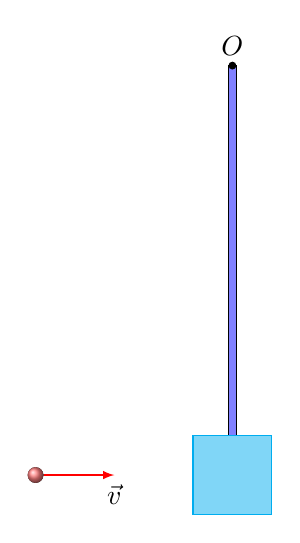
\begin{tikzpicture}
			\pgfmathsetmacro{\l}{5.2}
			\coordinate (O) at (0,0) node[above] {$O$};
			\draw[fill=blue!50] ([xshift=-0.05cm]O) rectangle +(0.1,-\l);
			\fill (0,0) coordinate (O) circle (0.05);
			\draw [cyan, fill=cyan!50] (-0.5,{-\l-0.5}) rectangle +(1,1);
			\draw[-latex, red] (-2.5,-\l) -- +(1,0) node[below, text=black] {$\vec v$};
			\fill[ball color = red!50] (-2.5,-\l) circle (0.1);
		\end{tikzpicture}
		\caption{Problem~\ref{prb:rot_bullet_ti_block}}
		\label{rot_bullet_ti_block}
	\end{minipage}
	%---------------------------------------------------------
	\begin{minipage}[t]{0.45\linewidth}\centering
		\begin{tikzpicture}
			\pgfmathsetmacro{\l}{5.5}
			\pgfmathsetmacro{\h}{3}
			\pgfmathsetmacro{\th}{0.1}
			\pgfmathsetmacro{\rang}{-45}
			\coordinate (O) at (0,0) node[above] {$O$};
			
			\draw[fill=blue!50] ([shift={(-\th/2,0)}]O) rectangle +(\th,-\l);
			\draw[fill=red, dashed] ({\th/2},-\l) rectangle +(0.4,0.4);
			
			\begin{scope}[opacity=0.5, rotate=\rang]
				\draw[fill=blue!50] ([shift={(-\th/2,0)}]O) rectangle +(\th,-\l);
				\draw[fill=red, dashed] ({\th/2},-\l) rectangle +(0.4,0.4);
			\end{scope}
			\draw (O) +(-90:0.5) arc (-90:{-90+\rang}:0.5) node[below, pos=0.7] {$\theta$};
			\fill (0,0) coordinate (O) circle (0.05);
			\draw[thick] (0,{-\l+\h}) +(-90:\h) arc(-90:0:\h);
			\draw[-latex] (0,{-\l+\h}) +(-25:{\h -0.2}) arc(-25:-45:{\h -0.2});
			\draw[fill=red] (0,{-\l+\h}) ++(0:\h) rectangle +(-0.4,-0.4);
			\node (wall) [ground, minimum width=8cm,yshift=-0.20cm] at (0,-\l) {};
			\draw (wall.north west) -- (wall.north east);
			\draw (\h,{-\l+\h}) -- +(0.5,0);
			\draw[latex-latex] ({\h +0.25},{-\l+\h}) -- node[fill=white] {$h$}+(0,-\h);
		\end{tikzpicture}
		\caption{Problem~\ref{prb:rot_block_hit_rod}}
		\label{rot_block_hit_rod}
	\end{minipage}
	%---------------------------------------------------------
\end{figure}
%=========================================================


%=========================================================
\begin{problem}\label{prb:ang_collision_particle_with_rod}
	\addpic{2}{0.5\linewidth}{%
		\captionsetup{type=figure}
			%---------------------------------------------------------
		\begin{subfigure}[t]{0.45\linewidth}\centering
			\begin{tikzpicture}
			\draw[blue, ultra thick] (2,2) -- node [left, text = black] {$O$}(2,-2);
			\node[pt=red] at (2,0) {};
			\draw [ultra thick, -latex] (0,2) -- +(1,0) node[below] {$\vec v_i$};
			\draw[ball color=red] (0,2)  node[above] {$m$} circle (0.1);
			\draw (2.1,2) -- +(1,0);		
			\draw (2.1,-2) -- +(1,0);
			\draw[latex-latex] (2.8,2) -- node[fill=white] {$d$} +(0,-4);
			\end{tikzpicture}
			\caption{}
			\label{ang_collision_particle_with_rod_a}
		\end{subfigure}
		\quad
		%---------------------------------------------------------
		\begin{subfigure}[t]{0.45\linewidth}\centering
			\begin{tikzpicture}
			\draw[blue, ultra thick] (2,2) -- node [left, text = black] {$O$}(2,-2);
			\node[pt=red] at (2,0) {};
			\draw[ball color=red] (1.9,2)  node[above] {$m$} circle (0.1);
			\draw[-latex, ultra thick, brown] (2,2) +(135:1) arc (135:45:1) node[right] {$\omega$};
			\end{tikzpicture}
			\caption{}
			\label{ang_collision_particle_with_rod_b}
		\end{subfigure}
		%---------------------------------------------------------
		\captionof{figure}{Problem~\ref{prb:ang_collision_particle_with_rod}}
	}[5]%
	A projectile of mass $m$ moves to the right with a speed $\vec v_i$ (Fig.~\ref{ang_collision_particle_with_rod_a}). The projectile strikes and sticks to the end of a stationary rod of mass $M$, length $d$, pivoted about a frictionless axle perpendicular to the page through $O$ (Fig.~\ref{ang_collision_particle_with_rod_b}).
	\begin{enumerate*}[label=(\alph*)]
		\item What is the angular momentum of the system before the collision about an axis through $O$?
		\item What is the moment of inertia (rotational inertia) of the system about an axis through $O$ after the projectile sticks to the rod?
		\item If the angular velocity of the system after the collision is $\omega$, what is the angular momentum of the system after the collision?
		\item Find the angular velocity $\omega$ after the collision in terms of the given quantities.
		\item What is the kinetic energy of the system before the collision?
		\item What is the kinetic energy of the system after the collision?
		\item Determine the fractional change of kinetic energy due to the collision.
	\end{enumerate*}
	\begin{solution}
		\begin{enumerate*}[label=(\alph*)]
			\item $\frac{mv_id}{2}$;
			\item $\left( \frac{M}{12} + \frac{m}{4}\right) d^2$;
			\item $\left( \frac{M}{12} + \frac{m}{4}\right) d^2\omega$;
			\item $\frac{6mv_i}{(M + 3m)d}$;
			\item $\frac{mv_i^2}{2}$;
			\item $\frac{3m^2v_i^2}{2(M + 3m)}$;
			\item $-\frac{M}{M + 3m}$.
		\end{enumerate*}
	\end{solution}
\end{problem}



\Closesolutionfile{answer}

